
\chapter{常に脚軌道生成が可能な自由歩容パターン生成手法を用いた実機実験}\label{chapter:常に脚軌道生成が可能な自由歩容パターン生成手法を用いた実機実験}

\chref{chapter:常に脚軌道生成が可能な自由歩容パターン生成手法を用いた実機実験}では,
実機を用いた歩行実験を行い,
本研究で提案した自由歩容パターン生成手法によって脚軌道生成の失敗が生じないことを示す.

\section{実験目的}
\chref{chapter:再評価手法の有効性の確認のための歩行シミュレーション}では,シミュレーションを用いて,
先行研究で歩行することができなかった地形で,脚軌道生成の失敗をすることなく歩行することができることを示した.
しかし,本研究で用いたシミュレーション環境では脚先の滑りによるずれやモータのトルクを考慮してない.
そのため,実機を用いた歩行実験を行い,
実際に本研究で提案した自由歩容パターン生成手法によって,
先行研究で歩行することができなかった地形で,歩行することができることを確認することを目的とする.

本章では,先行研究で歩行することができなかった130mmの段差の上りおよび下りを行い,
脚軌道生成の失敗をすることなく歩行することができることを示す.

\section{実験方法}
\subsection{歩行する地形}
ロボットが歩行する地形を\figref{fig:walking-terrain}に示す.
地形の材質には,滑りにくさや加工のしやすさなどの理由から,
建築用断熱材であるスタイロフォームを用いた.
また,地形は\figref{fig:walking-terrain}のように,右側が左側に比べて130mm高くなっている.
上り動作の際には左側から右側に向かって歩行させ,下り動作の際には右側から左側に向かって歩行させた.

% fig:walking-terrain
\begin{figure}[tb]
  \centering
  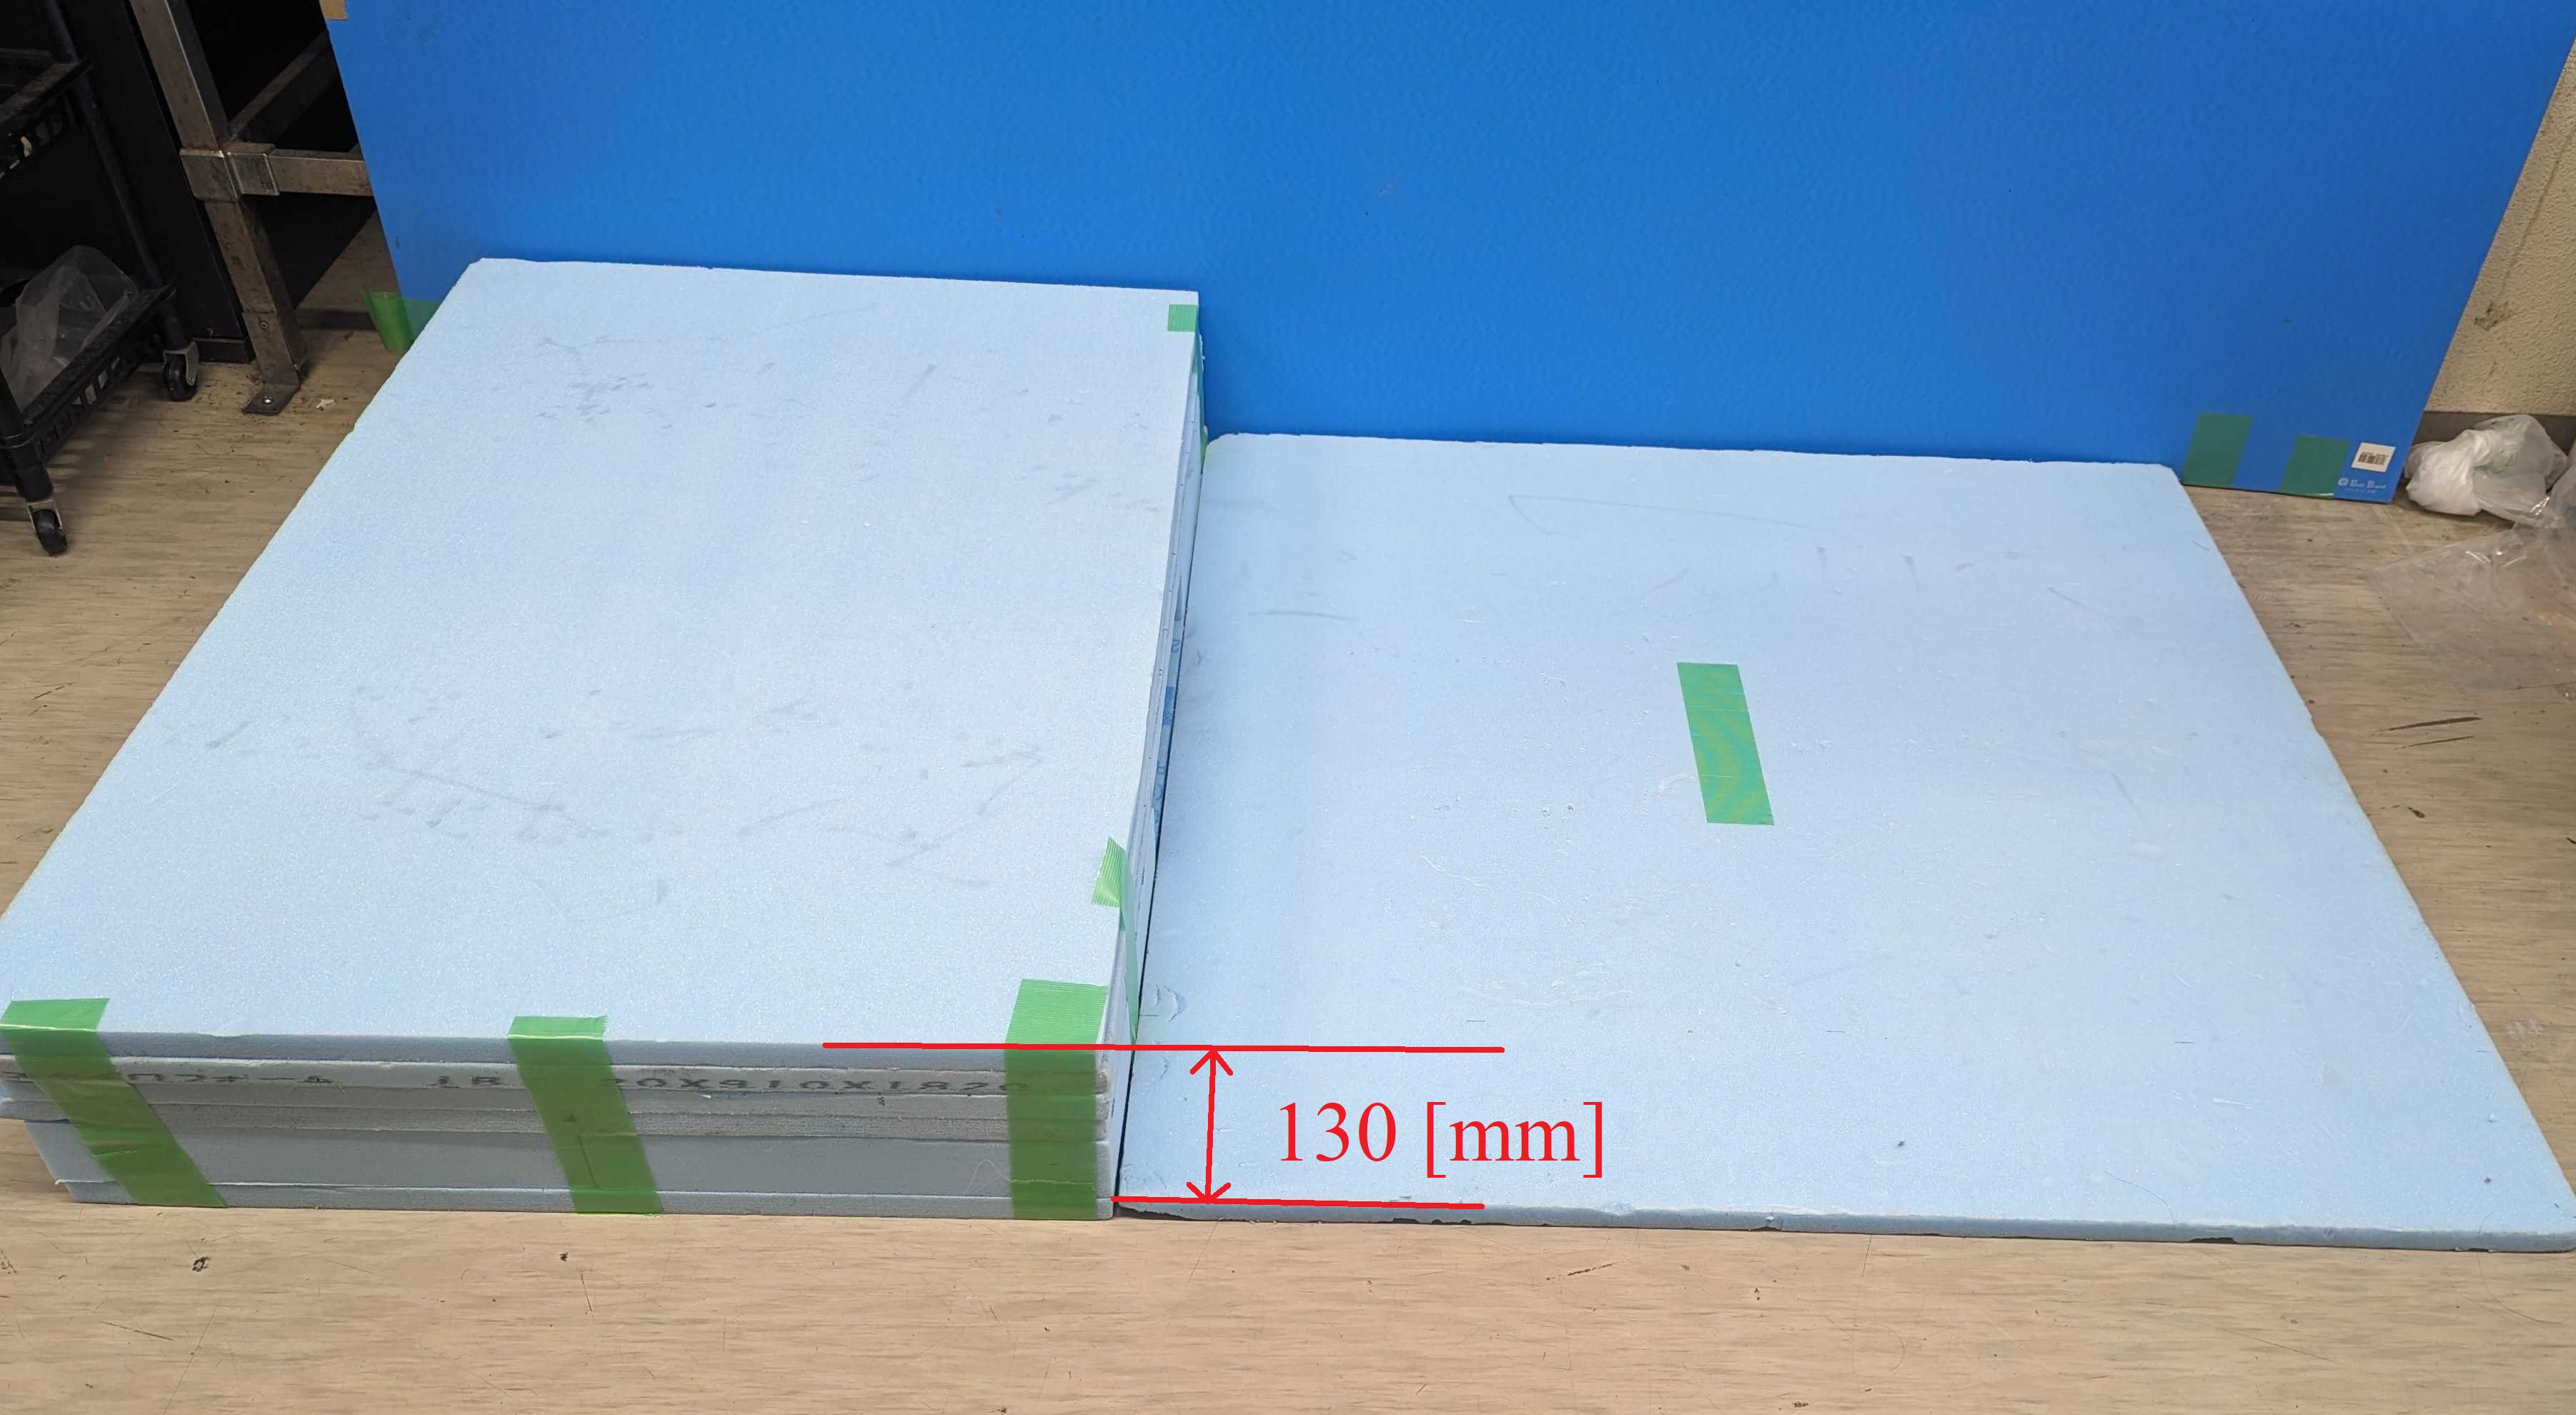
\includegraphics[width=0.8\linewidth]{figure/chapter5/walking-terrain.jpg}
  \caption{Walking Terrain}
  \label{fig:walking-terrain}  % chktex 24
\end{figure}

\subsection{使用したロボット}
実験ではシミュレーションのモデルとしていたPhantomXを使用した.
内部電源では長時間稼働させるには容量が足りないため,
電源には外部電源として安定化電源($12V,5A$)を使用した.
ロボットへの指令値は,グラフ探索による自由歩容パターン生成手法を用いてPCで計算し,
XBeeを用いてPhantomXに送信した.

ロボットの脚軌道は矩形軌道を用いた.
また,本実験は先行研究では歩行ができなかった地形で歩行ができることを示すことが目的であるため,
地形は既知のものとし,地形の形状をセンサで計測することは行わなかった.

\subsection{実験の条件}
歩行実験時の歩行条件を以下に示す.

\begin{itemize}
  \item 胴体姿勢は常に地面と水平にする
  \item 動作は直進動作のみを行う
  \item ロボットの重心からみた遊脚高さは-20mmとする
  \item 安定余裕を15mmとする
  \item 胴体は地形から30mm以上離す
\end{itemize}

また,グラフ探索の条件を以下に示す.

\begin{itemize}
  \item 探索するグラフの深さは5とする
  \item 近似された可動範囲の最小半径は140mmとする
\end{itemize}

\subsection{実験の手順}
まず,ロボットを段差の手前に配置した.
次に,130mmの段差を上りおよび下りするまでの自由歩容パターンを生成し,
ロボットにXBeeを通じて送信した.
そして,送信された指令値に基づいてロボットが歩行する様子を撮影した.
ロボットの6脚すべてが段差を乗り越えることができた場合に,
ロボットが段差を乗り越えたと判断した.

\section{結果}
130mmの段差を上る様子を\figref{fig:ch5_experiment_1}に示す.
この図は,ロボットが動作する様子をタイムラプスで撮影したものである.
30枚の写真で構成されており,初めから順番に01から30までの番号が右上に振られている.
この図から,ロボットが重心高さを変更し130mmの段差を上る様子が確認できる.
ロボットは最初,画面右側に配置されており,胴体高さを上げたのち,
段差の上に脚を接地して段差を上り,画面左側に向けて歩行している.

130mmの段差を下りる様子を\figref{fig:ch5_experiment_2}に示す.
この図も同様にタイムラプスで撮影している.
この図から,ロボットが重心高さを変更し130mmの段差を下る様子が確認できる.
ロボットは最初,画面左側に配置されており,段差の下へ胴体を乗り出しつつ脚を接地し,
段差を下ったのち胴体高さを下げて,画面右側に向けて歩行している.

以上より,130mmの上り段差および,130mmの下り段差の両方の地形で段差を乗り越えることに成功した.

\begin{figure}[h]
  \centering
  \includegraphics[width=0.7\linewidth]{figure/chapter5/up.png}
  \caption{Actual Equipment Experiment (130mm steps up)}
  \label{fig:ch5_experiment_1}  % chktex 24
\end{figure}

\begin{figure}[h]
  \centering
  \includegraphics[width=0.7\linewidth]{figure/chapter5/down.png}
  \caption{Actual Equipment Experiment (130mm steps down)}
  \label{fig:ch5_experiment_2}  % chktex 24
\end{figure}

\section{考察}
結果より先行研究で歩行することができなかった地形で,
脚軌道生成の失敗をすることなく歩行することができると確認できた.
これによって,先行研究の問題点であった脚軌道生成の失敗を解決することができると示された.

しかし実験の最中に,シミュレーションでは確認できなかったいくつかの課題があると確認された.
以下にそれらを列挙する.

\begin{itemize}
  \item 支持脚に滑りが生じる.
  \item トルク不足による胴体の沈み込みや傾きが生じる.
\end{itemize}

このような滑りや傾きによって,実際のロボットの座標と指令値に誤差が生じ,目的の座標へ脚先を移動できないことがあった.
支持脚の滑りや,脚のトルク不足による胴体の沈み込みが生じてしまうことは,
グラフ探索による自由歩容パターン生成手法ではロボットの脚先の摩擦や,モータのトルクを考慮していないため生じる問題である.
これを防ぐためには,ロボットの姿勢からトルクを計算し,脚のトルク不足が生じないようにする必要がある.
しかし,このような力学的な計算を行うことは,グラフ探索の処理時間を増加させるため,
ノードごとに計算を行うことは,現実的ではない.
よって,脚の静力学解析を行い,脚のトルク不足による胴体の沈み込みが起きない,
十分なトルクを出すことができる範囲を近似された可動範囲として設定する必要があるだろう.

